\section{Introduction}
\label{sec:intro}

\begin{tight_itemize}
  \item Introduce the problem
  \item Describe our approach
  \item Contrast with Milan's work
  \item Contrast with Andreas Geiger's work
  \item Highlight the contributions
\end{tight_itemize}
\vspace{10cm}
\begin{figure}[!!t]
  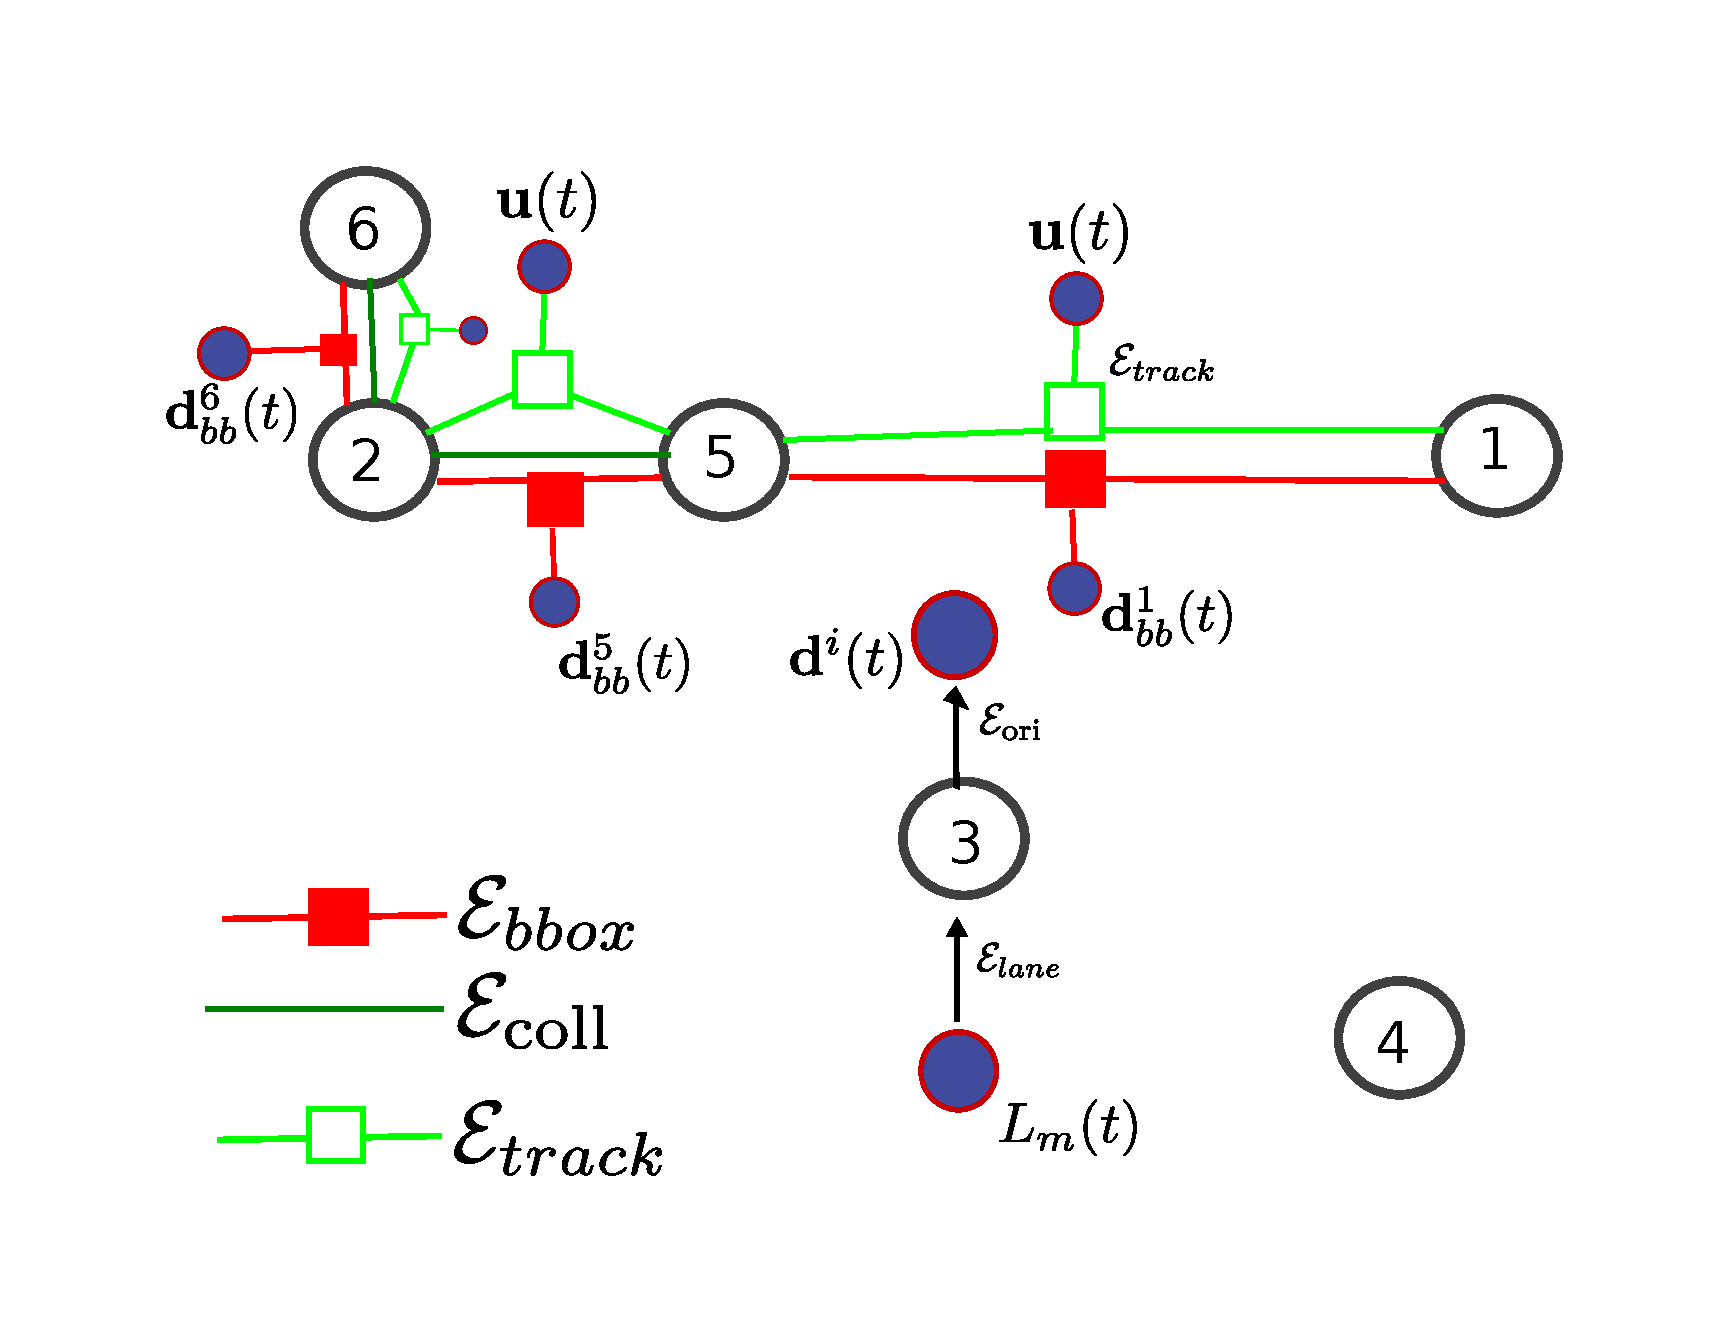
\includegraphics[width=\columnwidth]{Figures/graphicalModelFrom61ConstVars.pdf}
  \caption{Graphical model. The six numbered black circles represent the
    unknown state variables of each car. All other nodes in the graphical model
    are assumed
    observed variables. Consider each energy in the model one by one. (1)
    Bounding box energy: The bounding box energy without occlusion modeling is
    a unary term, but with occlusion it becomes a higher order term that
    affects the state of occluder as well. In this graphical model we assume
    that the scene is being observed from left to right, hence "2" occludes "6"
    and "5" and "5" occludes "1". The bounding box detection is represented by
  $\mathbf{d}_{bb}^i(t)$ and the statistical dependencies are represented by
  red lines. (2) Point tracks ($\Energy{track}$): Since occlusion is also
  included in modeling point tracks energy we have similar interdependencies
  for point tracks energy. The available point tracks are modeled by
  $\mathbf{u}(t)$. (3) Collision ($\Energy{coll}$) : The collision energy
  mathematically is a dense graph between all the TP but here we represent
  collision among only those TP that are near enough to have a significant
collision energy. (4) Orientation from detection ($\Energy{ori}$) (5) Orientation from lane (and map) information ($\Energy{lane}$)}
  \label{fig:graphmodel}
\end{figure}
\begin{figure}
  \centering
    	  \begin{tikzpicture}[grow cyclic,line width=1.2pt,
variablenode/.style={circle,circular drop shadow,draw=black,fill=green,thick,minimum width=1.0cm},
  	  factor/.style={rectangle,drop shadow,draw=black,fill=white,thick,minimum width=1.1cm},
      obs/.style={fill=gray!30},
      prev/.style={text=gray,draw=gray,fill=green!50}]
  	  \path 

(0.6,2.8) node [variablenode,prev] (xt1) {$x_{t-1}$}
(2.6,2.8) node [variablenode,prev] (theta1) {$\theta_{t-1}$}

(-0.05,1.8) node [factor,draw=gray,text=gray] (fdynx) {$E_{d}$}
(1.95,1.8) node [factor,draw=gray,text=gray,minimum width=1cm] (fdynt) {$E_{d}$}

(.7,1.1) node[factor](fhol) {$E_{hol}$}

  	 (1, 0)  node[variablenode](theta){$\theta_t$}
   [counterclockwise from=-60,sibling angle=60]
     (2.5, 0) node [factor] (flane) {$E_{lane}$} 
    child { node [variablenode,obs] (l) { $L_t$ } }
    child { node [ variablenode,obs,font=\footnotesize] (gps) {GPS}}
    child { node [ variablenode,obs,font=\footnotesize] (gps) {Map}}
  	(-1, 0)  node[variablenode](xt){$\mathbf{x}_t$}

    [counterclockwise from=60,sibling angle=60]
  	(-2, 1.5) node[factor](fdet){$E_{det}$} 
  	           child {
  	             node[variablenode,obs](gp){$G_t$} 
  	  			}
	  	   		child {           node[variablenode,obs](Det){$D_t$}
  			  }

      (-2.0,-1.5) node[factor](fsize){$E_{size}$}
     (-3,0) node[variablenode](dim){$B$}
[counterclockwise from=-90]
 (0, -1.5) node[factor](fpt) {$E_{pt}$}
 child { node[variablenode,obs](pt){$u_t$} }


  	  ;
  	  \draw (xt) -- (fdet) -- (Det);
  	  \draw (xt) edge (fpt);
      \draw (fpt) -- (pt);
  	  \path  (fpt) edge (theta);
  	  \draw (fdet) -- (gp);
      \draw (fhol) -- (xt);
      \draw (fhol) -- (xt1);
      \draw (fhol) -- (theta);  	  
      \draw (dim) -- (fdet);
     \draw (xt) -- (fsize) -- (dim);
   \draw (theta) -- (flane);
   \draw (xt) -- (fdynx) -- (xt1);
   \draw (theta) -- (fdynt) -- (theta1);
	\end{tikzpicture}

  
\end{figure}
